% Options for packages loaded elsewhere
\PassOptionsToPackage{unicode}{hyperref}
\PassOptionsToPackage{hyphens}{url}
\PassOptionsToPackage{dvipsnames,svgnames,x11names}{xcolor}
%
\documentclass[
  xelatex,
  ja=standard]{bxjsarticle}

\usepackage{amsmath,amssymb}
\usepackage{iftex}
\ifPDFTeX
  \usepackage[T1]{fontenc}
  \usepackage[utf8]{inputenc}
  \usepackage{textcomp} % provide euro and other symbols
\else % if luatex or xetex
  \usepackage{unicode-math}
  \defaultfontfeatures{Scale=MatchLowercase}
  \defaultfontfeatures[\rmfamily]{Ligatures=TeX,Scale=1}
\fi
\usepackage{lmodern}
\ifPDFTeX\else  
    % xetex/luatex font selection
  \setmainfont[BoldFont=Noto Sans CJK JP]{Noto Serif CJK JP}
\fi
% Use upquote if available, for straight quotes in verbatim environments
\IfFileExists{upquote.sty}{\usepackage{upquote}}{}
\IfFileExists{microtype.sty}{% use microtype if available
  \usepackage[]{microtype}
  \UseMicrotypeSet[protrusion]{basicmath} % disable protrusion for tt fonts
}{}
\makeatletter
\@ifundefined{KOMAClassName}{% if non-KOMA class
  \IfFileExists{parskip.sty}{%
    \usepackage{parskip}
  }{% else
    \setlength{\parindent}{0pt}
    \setlength{\parskip}{6pt plus 2pt minus 1pt}}
}{% if KOMA class
  \KOMAoptions{parskip=half}}
\makeatother
\usepackage{xcolor}
\setlength{\emergencystretch}{3em} % prevent overfull lines
\setcounter{secnumdepth}{5}
% Make \paragraph and \subparagraph free-standing
\ifx\paragraph\undefined\else
  \let\oldparagraph\paragraph
  \renewcommand{\paragraph}[1]{\oldparagraph{#1}\mbox{}}
\fi
\ifx\subparagraph\undefined\else
  \let\oldsubparagraph\subparagraph
  \renewcommand{\subparagraph}[1]{\oldsubparagraph{#1}\mbox{}}
\fi


\providecommand{\tightlist}{%
  \setlength{\itemsep}{0pt}\setlength{\parskip}{0pt}}\usepackage{longtable,booktabs,array}
\usepackage{calc} % for calculating minipage widths
% Correct order of tables after \paragraph or \subparagraph
\usepackage{etoolbox}
\makeatletter
\patchcmd\longtable{\par}{\if@noskipsec\mbox{}\fi\par}{}{}
\makeatother
% Allow footnotes in longtable head/foot
\IfFileExists{footnotehyper.sty}{\usepackage{footnotehyper}}{\usepackage{footnote}}
\makesavenoteenv{longtable}
\usepackage{graphicx}
\makeatletter
\def\maxwidth{\ifdim\Gin@nat@width>\linewidth\linewidth\else\Gin@nat@width\fi}
\def\maxheight{\ifdim\Gin@nat@height>\textheight\textheight\else\Gin@nat@height\fi}
\makeatother
% Scale images if necessary, so that they will not overflow the page
% margins by default, and it is still possible to overwrite the defaults
% using explicit options in \includegraphics[width, height, ...]{}
\setkeys{Gin}{width=\maxwidth,height=\maxheight,keepaspectratio}
% Set default figure placement to htbp
\makeatletter
\def\fps@figure{htbp}
\makeatother

\renewcommand{\thefootnote}{\arabic{footnote}}
\makeatletter
\@ifpackageloaded{tcolorbox}{}{\usepackage[skins,breakable]{tcolorbox}}
\@ifpackageloaded{fontawesome5}{}{\usepackage{fontawesome5}}
\definecolor{quarto-callout-color}{HTML}{909090}
\definecolor{quarto-callout-note-color}{HTML}{0758E5}
\definecolor{quarto-callout-important-color}{HTML}{CC1914}
\definecolor{quarto-callout-warning-color}{HTML}{EB9113}
\definecolor{quarto-callout-tip-color}{HTML}{00A047}
\definecolor{quarto-callout-caution-color}{HTML}{FC5300}
\definecolor{quarto-callout-color-frame}{HTML}{acacac}
\definecolor{quarto-callout-note-color-frame}{HTML}{4582ec}
\definecolor{quarto-callout-important-color-frame}{HTML}{d9534f}
\definecolor{quarto-callout-warning-color-frame}{HTML}{f0ad4e}
\definecolor{quarto-callout-tip-color-frame}{HTML}{02b875}
\definecolor{quarto-callout-caution-color-frame}{HTML}{fd7e14}
\makeatother
\makeatletter
\makeatother
\makeatletter
\makeatother
\makeatletter
\@ifpackageloaded{caption}{}{\usepackage{caption}}
\AtBeginDocument{%
\ifdefined\contentsname
  \renewcommand*\contentsname{目次}
\else
  \newcommand\contentsname{目次}
\fi
\ifdefined\listfigurename
  \renewcommand*\listfigurename{図一覧}
\else
  \newcommand\listfigurename{図一覧}
\fi
\ifdefined\listtablename
  \renewcommand*\listtablename{表一覧}
\else
  \newcommand\listtablename{表一覧}
\fi
\ifdefined\figurename
  \renewcommand*\figurename{図}
\else
  \newcommand\figurename{図}
\fi
\ifdefined\tablename
  \renewcommand*\tablename{表}
\else
  \newcommand\tablename{表}
\fi
}
\@ifpackageloaded{float}{}{\usepackage{float}}
\floatstyle{ruled}
\@ifundefined{c@chapter}{\newfloat{codelisting}{h}{lop}}{\newfloat{codelisting}{h}{lop}[chapter]}
\floatname{codelisting}{コード}
\newcommand*\listoflistings{\listof{codelisting}{コード一覧}}
\makeatother
\makeatletter
\@ifpackageloaded{caption}{}{\usepackage{caption}}
\@ifpackageloaded{subcaption}{}{\usepackage{subcaption}}
\makeatother
\makeatletter
\@ifpackageloaded{tcolorbox}{}{\usepackage[skins,breakable]{tcolorbox}}
\makeatother
\makeatletter
\@ifundefined{shadecolor}{\definecolor{shadecolor}{rgb}{.97, .97, .97}}
\makeatother
\makeatletter
\makeatother
\makeatletter
\makeatother
\ifLuaTeX
\usepackage[bidi=basic]{babel}
\else
\usepackage[bidi=default]{babel}
\fi
\babelprovide[main,import]{japanese}
% get rid of language-specific shorthands (see #6817):
\let\LanguageShortHands\languageshorthands
\def\languageshorthands#1{}
\ifLuaTeX
  \usepackage{selnolig}  % disable illegal ligatures
\fi
\usepackage[]{natbib}
\bibliographystyle{jecon}
\IfFileExists{bookmark.sty}{\usepackage{bookmark}}{\usepackage{hyperref}}
\IfFileExists{xurl.sty}{\usepackage{xurl}}{} % add URL line breaks if available
\urlstyle{same} % disable monospaced font for URLs
\hypersetup{
  pdftitle={現代の戦争と平和},
  pdfauthor={土井翔平},
  pdflang={ja},
  colorlinks=true,
  linkcolor={NavyBlue},
  filecolor={Maroon},
  citecolor={NavyBlue},
  urlcolor={NavyBlue},
  pdfcreator={LaTeX via pandoc}}

\title{現代の戦争と平和}
\usepackage{etoolbox}
\makeatletter
\providecommand{\subtitle}[1]{% add subtitle to \maketitle
  \apptocmd{\@title}{\par {\large #1 \par}}{}{}
}
\makeatother
\subtitle{国際公共政策学}
\author{土井翔平}
\date{2023-04-23}

\begin{document}
\maketitle
\ifdefined\Shaded\renewenvironment{Shaded}{\begin{tcolorbox}[sharp corners, interior hidden, borderline west={3pt}{0pt}{shadecolor}, boxrule=0pt, breakable, frame hidden, enhanced]}{\end{tcolorbox}}\fi

\hypertarget{ux306fux3058ux3081ux306b}{%
\section*{はじめに}\label{ux306fux3058ux3081ux306b}}
\addcontentsline{toc}{section}{はじめに}

平和は協調的な国際関係の前提となる。そこで、平和や戦争の要因を学ぶ。

\begin{itemize}
\tightlist
\item
  現代の戦争の特徴はなにか?
\item
  なぜ平和ではなく戦争が選択されるのか?
\end{itemize}

\hypertarget{ux4e16ux754cux306bux304aux3051ux308bux7d1bux4e89ux66b4ux529b}{%
\section{世界における紛争・暴力}\label{ux4e16ux754cux306bux304aux3051ux308bux7d1bux4e89ux66b4ux529b}}

武力紛争を定義し、データセットを構築して、数える試み\citep[序章]{tago2020}

\begin{itemize}
\tightlist
\item
  \href{https://www.cao.go.jp/pko/pko_j/organization/researcher/atpkonow/article099.html}{紛争に関するデータセット}
\end{itemize}

\hypertarget{ux7d1bux4e89ux306eux983bux5ea6ux3068ux5f62ux614b}{%
\subsection{紛争の頻度と形態}\label{ux7d1bux4e89ux306eux983bux5ea6ux3068ux5f62ux614b}}

どのような紛争が、どの程度発生しているのか?

\href{https://ucdp.uu.se/encyclopedia}{Uppsala Conflict Data Program
(UCDP)} のデータ\citep{gleditsch2002}

\begin{tcolorbox}[enhanced jigsaw, title=\textcolor{quarto-callout-note-color}{\faInfo}\hspace{0.5em}{\href{https://ucdp.uu.se/downloads/ucdpprio/ucdp-prio-acd-221.pdf}{UCDPにおける武力紛争の定義}}, colbacktitle=quarto-callout-note-color!10!white, bottomtitle=1mm, coltitle=black, titlerule=0mm, colback=white, rightrule=.15mm, toprule=.15mm, opacityback=0, breakable, opacitybacktitle=0.6, toptitle=1mm, arc=.35mm, leftrule=.75mm, bottomrule=.15mm, left=2mm, colframe=quarto-callout-note-color-frame]

UCDP defines state-based armed conflict as: ``a \textbf{contested
incompatibility} that concerns government and/or territory where the
\textbf{use of armed force} between \textbf{two parties}, of which at
least one is the government of a state, results in at least \textbf{25
battle-related deaths} in a calendar year.''

\end{tcolorbox}

\begin{figure}[htpb]

{\centering 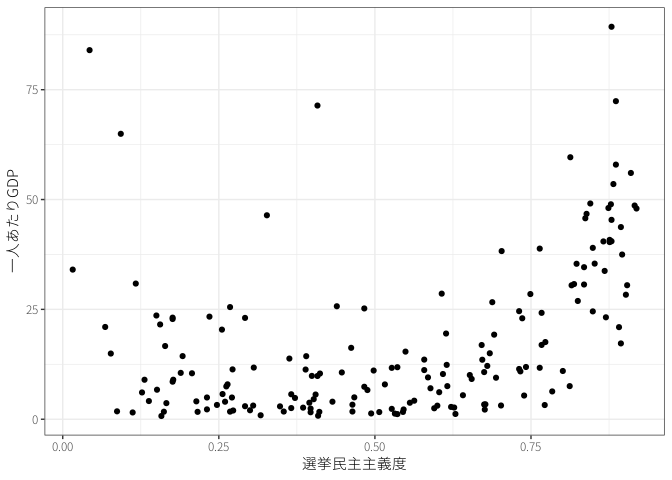
\includegraphics{war_and_peace_files/figure-pdf/unnamed-chunk-2-1.png}

}

\caption{武力紛争 (UCDP) の発生件数}

\end{figure}

\begin{figure}[htpb]

{\centering 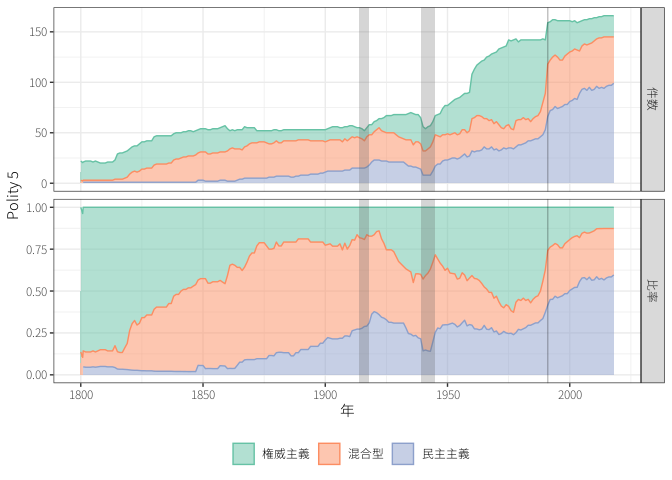
\includegraphics{war_and_peace_files/figure-pdf/unnamed-chunk-3-1.png}

}

\caption{武力紛争 (UCDP) の種類}

\end{figure}

\(\leadsto\)内戦の時代?

\href{https://correlatesofwar.org/data-sets/MIDs}{Correlates of War
(COW)} のデータ\citep{palmer2022}

\begin{itemize}
\tightlist
\item
  No militarized action
\item
  Threat to use force
\item
  Display use of force
\item
  Use of force, War
\end{itemize}

\begin{figure}[htpb]

{\centering 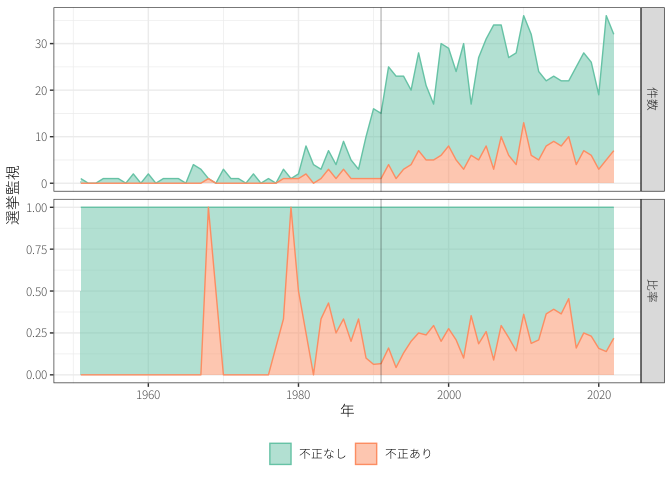
\includegraphics{war_and_peace_files/figure-pdf/unnamed-chunk-4-1.png}

}

\caption{国家間武力衝突 (MID) の発生件数}

\end{figure}

\begin{figure}[htpb]

{\centering 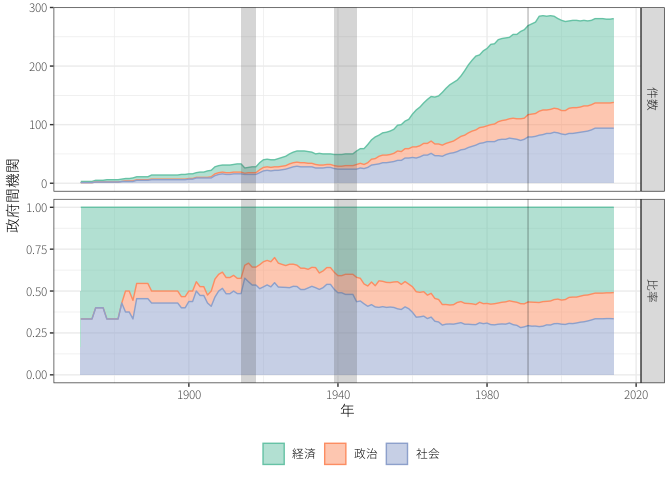
\includegraphics{war_and_peace_files/figure-pdf/unnamed-chunk-5-1.png}

}

\caption{国家間武力衝突 (MID) の種類}

\end{figure}

\begin{figure}[htpb]

{\centering 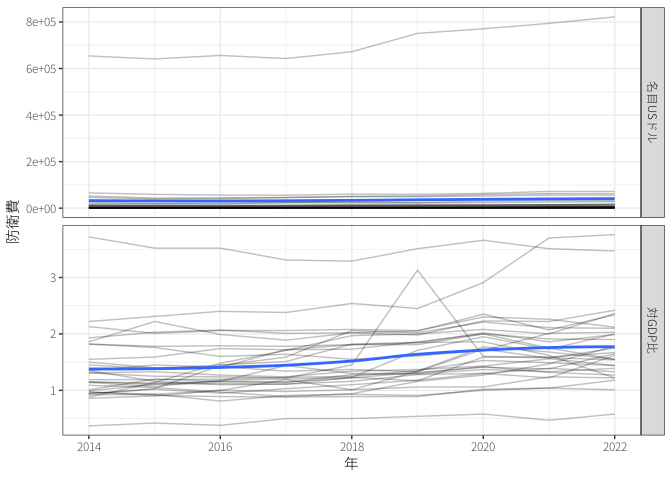
\includegraphics{war_and_peace_files/figure-pdf/unnamed-chunk-6-1.png}

}

\caption{国家間武力衝突 (MID) の当事国の割合}

\end{figure}

\hypertarget{ux7d1bux4e89ux306eux539fux56e0}{%
\subsection{紛争の原因}\label{ux7d1bux4e89ux306eux539fux56e0}}

なにを巡って集団は争うのか?

\begin{figure}[htpb]

{\centering 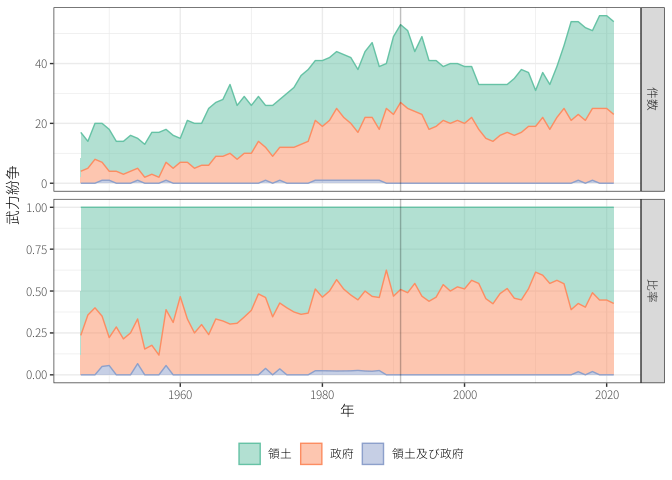
\includegraphics{war_and_peace_files/figure-pdf/unnamed-chunk-7-1.png}

}

\caption{武力紛争 (UCDP) の対立理由}

\end{figure}

\hypertarget{ux66b4ux529bux306eux7a7aux9593ux7684ux5206ux5e03}{%
\subsection{暴力の空間的分布}\label{ux66b4ux529bux306eux7a7aux9593ux7684ux5206ux5e03}}

どのような国や地域で紛争は頻発しているのか?

\begin{figure}[htpb]

{\centering 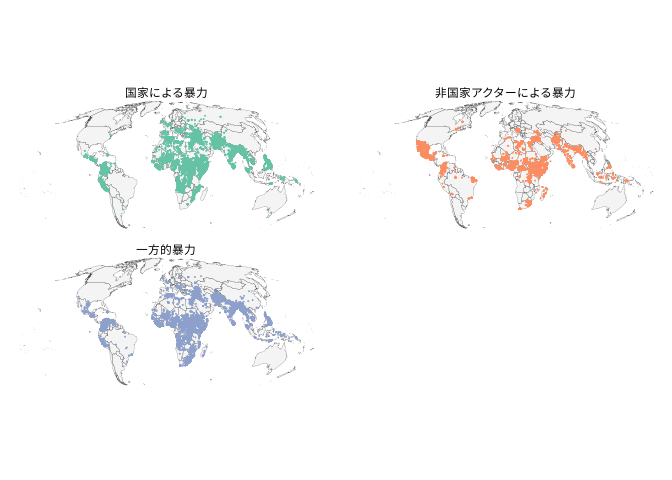
\includegraphics{war_and_peace_files/figure-pdf/unnamed-chunk-8-1.png}

}

\caption{暴力 (UCDP) の発生場所}

\end{figure}

\hypertarget{ux6226ux4e89ux3068ux5e73ux548cux306bux3064ux3044ux3066ux8003ux3048ux308bux610fux7fa9}{%
\section{戦争と平和について考える意義}\label{ux6226ux4e89ux3068ux5e73ux548cux306bux3064ux3044ux3066ux8003ux3048ux308bux610fux7fa9}}

国家間紛争が珍しい時代に安全保障について考える意義とは?

\begin{itemize}
\tightlist
\item
  (悲しいことに)2022年以降は当たり前のことかもしれない。
\item
  これまで平和であった\(\neq\)今後も平和である?
\item
  安全保障で現れる問題は、内戦やテロリズム、国際政治経済においても現れる。
\end{itemize}

国際関係論の始まり?

\begin{itemize}
\tightlist
\item
  古代ギリシャのトゥキュディデスが書いた「戦史」\citep{thucydides2013}
\item
  1939年に出版されたE.H.カーの「危機の二十年」\citep{carr2011}
\end{itemize}

戦争とは被害がある(社会的に効率的ではない)。

\hypertarget{ux8ecdux4e8bux652fux51fa}{%
\subsection{軍事支出}\label{ux8ecdux4e8bux652fux51fa}}

なぜ軍事支出を増やすのか?

\href{https://sipri.org/}{Stockholm International Peace Research
Institute}のデータ

\begin{figure}[htpb]

{\centering 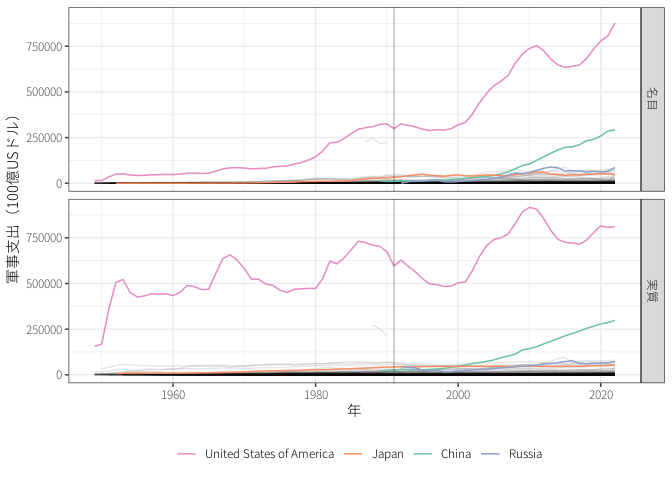
\includegraphics{war_and_peace_files/figure-pdf/unnamed-chunk-9-1.png}

}

\caption{軍事支出 (SIPRI) の推移}

\end{figure}

\begin{figure}[htpb]

{\centering 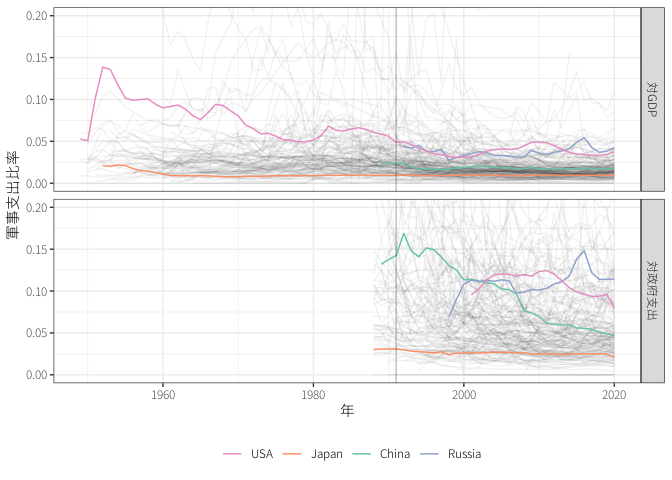
\includegraphics{war_and_peace_files/figure-pdf/unnamed-chunk-10-1.png}

}

\caption{軍事支出 (SIPRI) のGDP比の推移}

\end{figure}

\hypertarget{ux6226ux4e89ux306eux88abux5bb3}{%
\subsection{戦争の被害}\label{ux6226ux4e89ux306eux88abux5bb3}}

戦争ではどの程度の犠牲者が出ているのか?

\begin{figure}[htpb]

{\centering 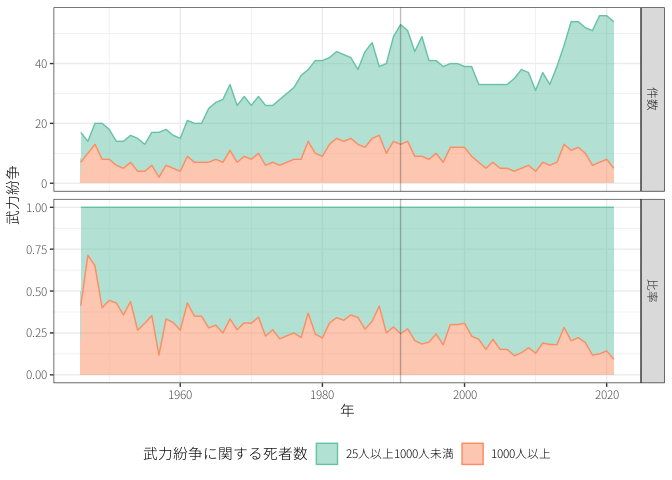
\includegraphics{war_and_peace_files/figure-pdf/unnamed-chunk-11-1.png}

}

\caption{武力衝突 (UCDP) の規模}

\end{figure}

\begin{figure}[htpb]

{\centering 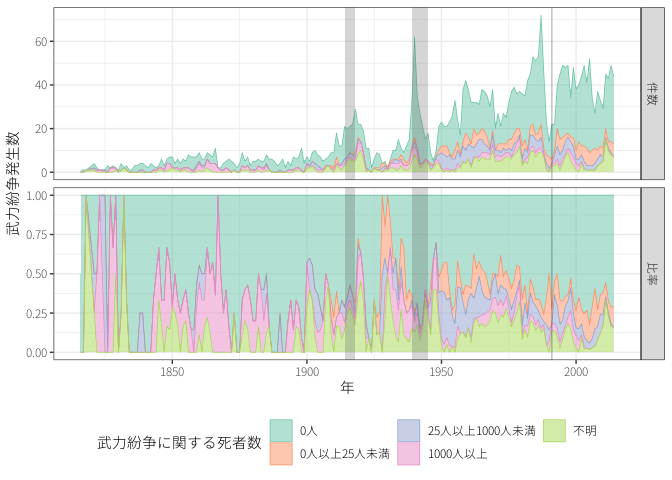
\includegraphics{war_and_peace_files/figure-pdf/unnamed-chunk-12-1.png}

}

\caption{国家間軍事衝突 (COW) の規模}

\end{figure}

\begin{figure}[htpb]

{\centering 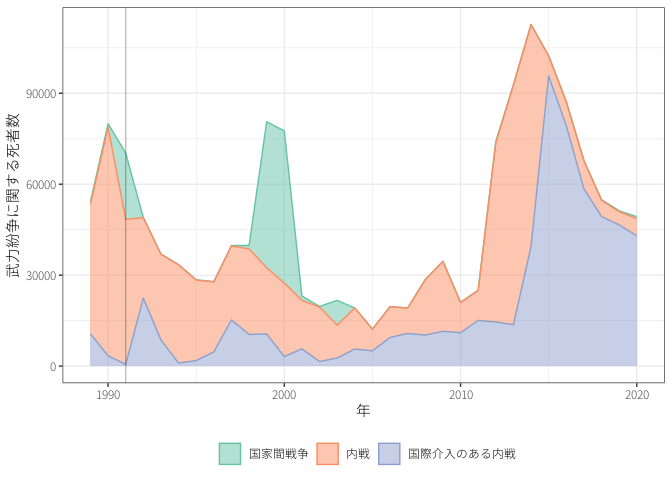
\includegraphics{war_and_peace_files/figure-pdf/unnamed-chunk-13-1.png}

}

\caption{武力衝突 (UCDP) の形態と被害者数の推移}

\end{figure}

\begin{figure}[htpb]

{\centering 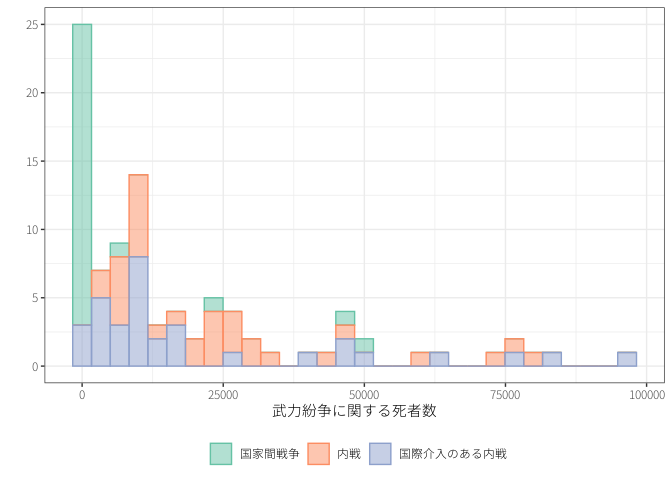
\includegraphics{war_and_peace_files/figure-pdf/unnamed-chunk-14-1.png}

}

\caption{武力衝突 (UCDP) の形態と被害者数}

\end{figure}

\begin{figure}[htpb]

{\centering 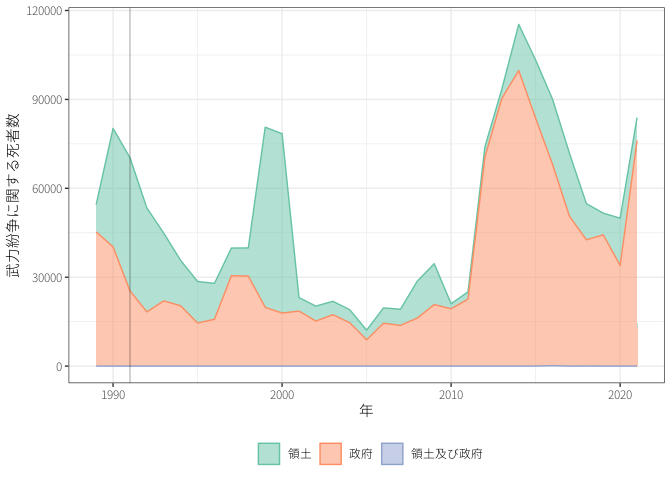
\includegraphics{war_and_peace_files/figure-pdf/unnamed-chunk-15-1.png}

}

\caption{武力衝突 (UCDP) の対立理由と被害者数の推移}

\end{figure}

\begin{figure}[htpb]

{\centering 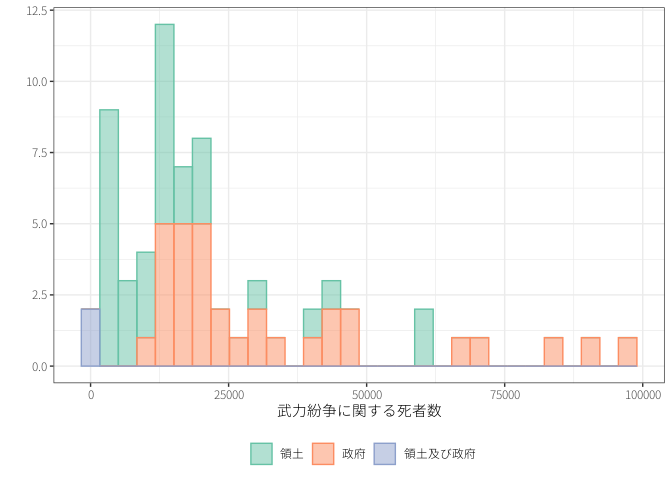
\includegraphics{war_and_peace_files/figure-pdf/unnamed-chunk-16-1.png}

}

\caption{武力衝突 (UCDP) の形態と被害者数}

\end{figure}

\hypertarget{ux6226ux4e89ux306eux671fux9593}{%
\subsection{戦争の期間}\label{ux6226ux4e89ux306eux671fux9593}}

\begin{figure}[htpb]

{\centering 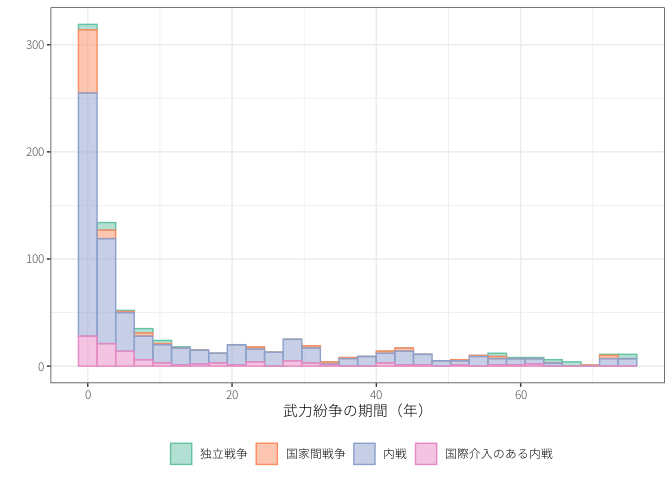
\includegraphics{war_and_peace_files/figure-pdf/unnamed-chunk-17-1.png}

}

\caption{武力衝突 (UCDP) の形態と期間}

\end{figure}

\begin{figure}[htpb]

{\centering 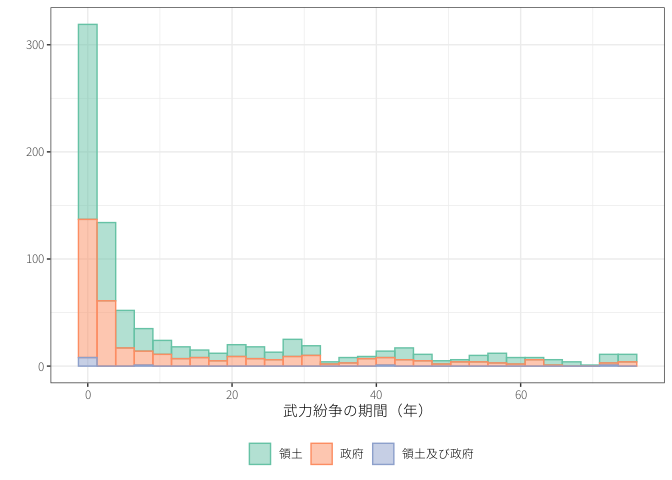
\includegraphics{war_and_peace_files/figure-pdf/unnamed-chunk-18-1.png}

}

\caption{武力衝突 (UCDP) の対立原因と期間}

\end{figure}

(人を殺してはいけないという一般的道徳以外に)なぜ戦争は望ましくないのか?

\(\leadsto\)戦争には損失(軍事費\footnote{軍事費の分だけ他の目的(例えば社会福祉)に予算を支出できないという意味で\textbf{機会費用}が発生する。}、犠牲者)がある=社会的に非効率的
(inefficient) \footnote{(非)効率性は経済学の概念であるが、ここでは無駄な資源の浪費があるという意味で理解されたい。}である。

\hypertarget{ux3082ux3046ux4e00ux3064ux306eux5e73ux548c}{%
\section{もう一つの平和}\label{ux3082ux3046ux4e00ux3064ux306eux5e73ux548c}}

\textbf{消極的平和} (negative peace):「戦争が存在しない状態」という平和
(peace)

\textbf{積極的平和} (positive
peace)\footnote{日本政府の提唱する\href{https://www.mofa.go.jp/mofaj/p_pd/dpr/page1w_000072.html}{積極的平和主義}とは、英訳するとProactive
  Contribution to Peaceであり、積極的平和とは異なる。}:「構造的暴力が存在しない状態」\citep{galtung1969, galtung1991}

\begin{itemize}
\tightlist
\item
  ヨハン・ガルトゥングは平和をより広く捉えた。
\item
  構造的暴力:軍事力に限らない貧困や抑圧、差別といった社会的不正義
\end{itemize}

安全保障 (security) の定義は困難

\begin{itemize}
\tightlist
\item
  主体、守るべき価値、脅威、手段から捉えられる\citep[第1章]{boudai2018}
\item
  軍事的安全保障や\textbf{伝統的安全保障}:国家が軍事力により軍事的脅威から国土や市民を守ること
\item
  \textbf{非伝統的安全保障}:非軍事的な脅威に対する安全保障

  \begin{itemize}
  \tightlist
  \item
    例えば、経済安全保障、エネルギー安全保障、食糧安全保障、気候安全保障など\(\leadsto\)結果として手段も非軍事的手段が主
  \item
    \href{https://www.mofa.go.jp/mofaj/gaiko/oda/bunya/security/index.html}{\textbf{人間の安全保障}}
    (human
    security):日本政府などは守るべき価値を国家ではなく人間として捉え直し、「生存・生活・尊厳に対する広範かつ深刻な脅威」から守るべきとすると提唱\citep{hs2003, sen2006, osa2021}
  \end{itemize}
\end{itemize}

この授業では軍事的な意味での平和や安全保障について学ぶ


  \bibliography{references.bib}


\end{document}
